


% =============================================================================
% ================================================================ Header Stuff
% =============================================================================

\documentclass{beamer}
\usepackage[utf8]{inputenc}
\usepackage{epsfig} % Allows the inclusion of eps files
\usepackage{epic} % Enhanced picture mode
\usepackage{eepic} % Extensions for epic
\usepackage{units} % SI unit typesetting
\usepackage{url} % URL handling
\usepackage{longtable} % Tables that continue onto multiple pages
\usepackage{mathrsfs} % Support for \mathscr script
\usepackage{multirow} % Span rows in tables
\usepackage{amssymb} % AMS math symbols and helpers
\usepackage{graphicx} % Enhanced graphics support
\usepackage{setspace} % Adjust spacing in captions, single by default
\usepackage{xspace} % Automatically adjusting space after macros
\usepackage{amsmath} % \text, and other math formatting options
\usepackage{siunitx} % \num{} formatting and SI unit formatting
\usepackage{booktabs} % Enhanced tables with \toprule, etc.
\usepackage{hyperref} % Add clickable links to other parts of the document
\usepackage[noabbrev,capitalize]{cleveref} % Automatically determine \cref type
\usepackage[hang,flushmargin]{footmisc} % Prevent indent in footnotes. 
\usepackage{xcolor} % so we can put todo notes in color. 
\usepackage{parskip} % http://ctan.org/pkg/parskip vskip instead of indent. 
\usepackage{float} % Sometimes you want to tell LaTeX to put an image RIGHT HERE. 
% Prevent LaTeX from putting a figure right before the start of a section. 
\usepackage[section]{placeins}
\usepackage[percent]{overpic}

% Try to prevent widows and orphans -- dangling parts of paragraphs over page breaks. 
\widowpenalty10000
\clubpenalty10000
% Configure the siunitx package
\sisetup{
    group-separator = {,}, % Use , to separate groups of digits, like 12,345
    list-final-separator = {, and } % Always use the serial comma in \SIlist
}
% Configure the cleveref package
\newcommand{\creflastconjunction}{, and } % Always use the serial comma



\newcommand{\Alfven}{Alfv\'en\xspace}

\newcommand{\Ampere}{Amp\`ere\xspace}

\newcommand{\xhat}{\ensuremath{\hat{x}}\xspace}
\newcommand{\yhat}{\ensuremath{\hat{y}}\xspace}
\newcommand{\zhat}{\ensuremath{\hat{z}}\xspace}

\DeclareSIUnit\RE{R_E}

\renewcommand{\vec}[1]{\underline{#1}}

\newcommand{\tensor}[1]{\underline{\underline{#1}}}

\newcommand{\dd}[1]{\ensuremath{ \frac{\partial}{\partial #1} }\xspace}

\newcommand{\ddt}{\dd{t}\xspace}

\newcommand{\dt}{\ensuremath{\delta \hspace{-0.1em} t} \xspace}

\newcommand{\curl}[1]{\ensuremath{ \nabla \times \vec{#1} }\xspace}

\newcommand{\lr}[1]{ \left( #1 \right) }

\newcommand{\lrsmall}[1]{ \left( {\scriptstyle #1} \right) }

\renewcommand{\arg}[1]{\!\lr{#1}}

\newcommand{\argsmall}[1]{\!\lrsmall{#1}}



\newcommand{\mmm}[9]{ \left[ \begin{array}{ccc}
    #1 & #2 & #3 \\
    #4 & #5 & #6 \\
    #7 & #8 & #9
  \end{array} \right] }

\newcommand{\mm}[4]{ \left[ \begin{array}{cc}
    #1 & #2 \\
    #3 & #4
  \end{array} \right] }

\newcommand{\vv}[2]{ \left[ \begin{array}{c}
    #1 \\
    #2
  \end{array} \right] }






% Note: Do we want to squish dt together? Do we want to always have tiny spaces
% between variables being multiplied together? 
\newcommand{\deltat}{\delta \hspace{-0.1em} t}


% Physics constants
\newcommand{\C}{{\mathrm{c}}}

% Add space between rows of tables
\newcommand{\spacerows}[1]{\renewcommand{\arraystretch}{#1}}

% Define a better looking eV by moving the V slightly left
\DeclareSIUnit\electronvolt{e\hspace{-0.08em}V}


\AtBeginSection[]{
  \begin{frame}
  \vfill
  \centering
  \begin{beamercolorbox}[sep=8pt,center,shadow=true,rounded=true]{title}
    \usebeamerfont{title}\insertsectionhead\par%
  \end{beamercolorbox}
  \vfill
  \end{frame}
}

% =============================================================================
% ============================================================== Begin Document
% =============================================================================

\title[FLR in 2.5D]{Field Line Resonance in Two and a Half Dimensions}
%\subtitle{PhD Defense}
%\institute{University of Minnesota}
\author{Charles McEachern}
\date{28 April 2016}

\usetheme{Boadilla}

\usefonttheme{serif}

\begin{document}

% =============================================================================
% ================================================================= Title Slide
% =============================================================================

\frame{\titlepage}

% =============================================================================
% ================================================================ Introduction
% =============================================================================

\section{Introduction}

% -----------------------------------------------------------------------------
% -----------------------------------------------------------------------------
% -----------------------------------------------------------------------------

\begin{frame}
\frametitle{Earth's Magnetic Field}

When shaken by the solar wind, etc, Earth's magnetic field lines rattle. 

\vfill

\begin{overpic}[width=0.6885\textwidth]{figures/nasa_magnetosphere.jpg}
 \put (0, 1) {\tiny\textcolor{white}{\;NASA}}
\end{overpic}%
\begin{overpic}[width=0.3115\textwidth]{figures/flora_borsi.jpg}
 \put (0, 1) {\tiny\textcolor{white}{\;Fl{\'o}ra Borsi}}
\end{overpic}%

\end{frame}

% -----------------------------------------------------------------------------
% -----------------------------------------------------------------------------
% -----------------------------------------------------------------------------

\begin{frame}
\frametitle{\Alfven Waves}

\begin{columns}
\column{0.5\textwidth}
\begin{wideitemize}
\item Shear \Alfven waves carry energy along magnetic field lines. 
\item Compressional \Alfven waves can carry energy across field lines. 
\item A field line resonance (FLR) is a shear \Alfven wave that fills the field line exactly. 
\end{wideitemize}
\column{0.5\textwidth}
\begin{overpic}[width=\textwidth]{figures/kv_alfven.png}
 \put (0, 1) {\tiny\textcolor{black}{\;Kivelson and Russell}}
\end{overpic}%
\end{columns}

\end{frame}

% -----------------------------------------------------------------------------
% -----------------------------------------------------------------------------
% -----------------------------------------------------------------------------

\begin{frame}
\frametitle{Characterizing Field Line Resonances}

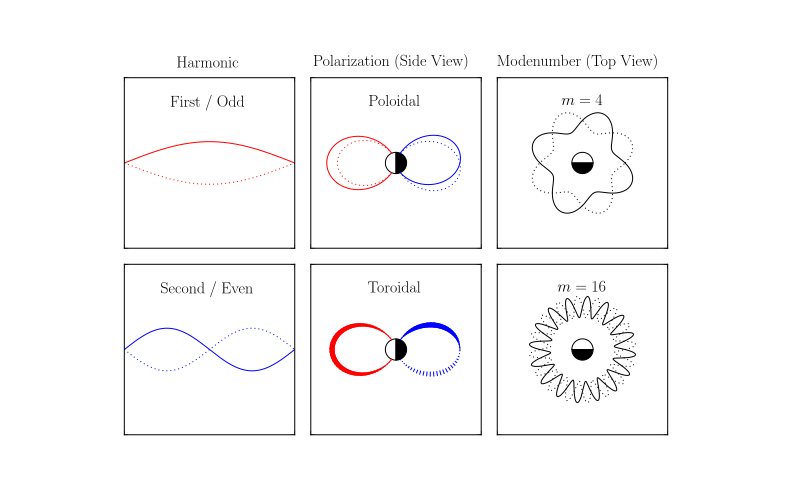
\includegraphics[width=\textwidth]{figures/properties.pdf}

\end{frame}

% -----------------------------------------------------------------------------
% -----------------------------------------------------------------------------
% -----------------------------------------------------------------------------

\begin{frame}
\frametitle{Poloidal-to-Toroidal Rotation}

\begin{columns}
\column{0.5\textwidth}
\begin{overpic}[width=\textwidth]{figures/mann_1995.png}
 \put (0, 1) {\tiny\textcolor{black}{\;Mann and Wright, 1995}}
\end{overpic}%
\column{0.5\textwidth}
\begin{wideitemize}
\item Poloidal FLRs rotate over time to become toroidal. 
\item The rotation is slower at large \azm. 
\item Toroidal FLRs do not rotate back. 
\end{wideitemize}
\end{columns}

\end{frame}

% -----------------------------------------------------------------------------
% -----------------------------------------------------------------------------
% -----------------------------------------------------------------------------

\begin{frame}
\frametitle{Pc4s and Giant Pulsations}

\begin{wideitemize}
\item Pc4 pulsations are resonant at auroral latitudes. 
\item They interact with trapped energetic particles. 
\item Giant pulsations are a small, distinctive subset of Pc4s.  
\end{wideitemize}

\vfill

\begin{center}
IAGA Frequency Bands [Jacobs, 1964]
\begin{tabular}{ @{\extracolsep{\fill}} cccccc @{\extracolsep{\fill}} }
  \hline
  & Pc1 & Pc2 & Pc3 & Pc4 & Pc5 \\
  \hline
  Period (\si{\second}) & 0.2--5    & 5--10    & 10--45  & 45--150 & 150--600 \\
  Frequency (\si{\mHz}) & 200--5000 & 100--200 & 22--100 & 7--22   & 2--7     \\
  \hline
\end{tabular}
\end{center}

\end{frame}

% =============================================================================
% ======================================================================= Model
% =============================================================================

\section{Numerical Model}

% -----------------------------------------------------------------------------
% -----------------------------------------------------------------------------
% -----------------------------------------------------------------------------

\begin{frame}
\frametitle{``Tuna Half'' Dimensional Grid}

\begin{columns}
\column{0.5\textwidth}
\begin{wideitemize}
\item Near Earth, at high \azm, 3D is too expensive. 
\item Earthward boundary is important for Pc4s --- keep it realistic. 
\item Simplifying assumption: everything goes as $\exp\arg{i \azm \phi}$. 
\item Grid is 2D, but fields and curls are 3D vectors. 
\end{wideitemize}
\column{0.5\textwidth}
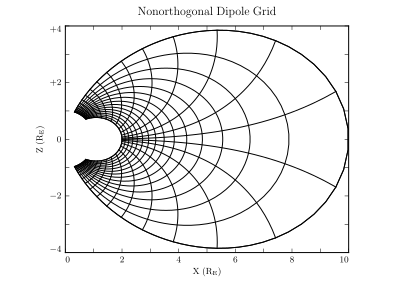
\includegraphics[width=\textwidth]{figures/grid.pdf}
\end{columns}

\end{frame}

% -----------------------------------------------------------------------------
% -----------------------------------------------------------------------------
% -----------------------------------------------------------------------------

\begin{frame}
\frametitle{Physical Parameter Profiles}

\begin{wideitemize}
\item Height-resolved conductivity from Kelley, modified by Lysak. 
\item Plasma density, including the plasmasphere. 
\item Four profiles: active day, quiet day, active night, quiet night. 
\end{wideitemize}

\vfill

\includegraphics[width=0.5\textwidth]{figures/va_2.pdf}%
\includegraphics[width=0.5\textwidth]{figures/fa_2.pdf}%

\end{frame}

% -----------------------------------------------------------------------------
% -----------------------------------------------------------------------------
% -----------------------------------------------------------------------------

\begin{frame}
\frametitle{Driving}

\begin{wideitemize}
\item At high \azm, driving at the outer boundary doesn't work. 
\item Tuna drives by perturbing the ring current instead. 
\item Magnitude is estimated from Sym-H storm index. 
\end{wideitemize}

\vfill

\includegraphics[width=\textwidth]{figures/drivers.pdf}%

\end{frame}

% -----------------------------------------------------------------------------
% -----------------------------------------------------------------------------
% -----------------------------------------------------------------------------

\begin{frame}
\frametitle{Maxwell's Equations}

Magnetic fields are updated using \farlaw:
\begin{align*}
  \tfrac{\partial}{\partial t} \vec{B} &= -\curl{E} &
  & \text{so} &
  \vec{B} &\assign \vec{B} - \dt \, \curl{E}
\end{align*}

Electric fields are updated using \amplaw and \ohmlaw:
\begin{align*}
  \tensor{\epsilon} \cdot \tfrac{\partial}{\partial t} \vec{E} = \tfrac{1}{\mz} \curl{B} - \vec{J} - \tensor{\sigma} \cdot \vec{E}
\end{align*}

Let $ \quad \tensor{V}^2 \equiv \frac{1}{\mz} \tensor{\epsilon}^{-1} \quad $ and $ \quad \tensor{\Omega} \equiv \tensor{\epsilon}^{-1} \cdot \tensor{\sigma} \quad $ so
\begin{align*}
  \lr{ \tensor{\Omega} + \tensor{ \mathbb{I} } \tfrac{\partial}{\partial t} } \cdot \vec{E} &= \tensor{V}^2 \cdot \big( \curl{B} - \mz \vec{J} \big)
\end{align*}

Which can be solved with an integrating factor: 
\begin{align*}
  \vec{E} &\assign \exp \arg{ -\tensor{\Omega} \, \dt } \cdot \vec{E} +
    \dt \, \exp \arg{ -\tensor{\Omega} \, \tfrac{\dt}{2} } \cdot
    \tensor{V}^2 \cdot \big( \curl{B} - \mz \vec{J} \big)
\end{align*}

\end{frame}

% -----------------------------------------------------------------------------
% -----------------------------------------------------------------------------
% -----------------------------------------------------------------------------

\begin{frame}
\frametitle{Coupling to the Atmosphere}

\begin{wideitemize}
\item Assume a perfectly-insulating atmosphere: $\curl{B} = 0$.  
\item From Maxwell's equations, $\div{B} = 0$. 
\item Then $\nabla^2\Psi = 0$ where $\nabla \Psi = \vec{B}$. 
\item Solution at the top of the atmosphere is a boundary condition:
\begin{align*}
  \tensor{\Sigma} \cdot \vec{E} &= \frac{1}{\mz} \,
    \displaystyle\lim_{\dr \rightarrow 0} \, \bigg[ \, \hat{r} \times \vec{B}
    \, \bigg|^{R_I + \dr}_{R_I - \dr}
\end{align*}
\item Solution at the bottom of the atmosphere gives ground signatures. 
\end{wideitemize}

\end{frame}

% =============================================================================
% ===================================================================== Results
% =============================================================================

\section{Numerical Results}

% -----------------------------------------------------------------------------
% -----------------------------------------------------------------------------
% -----------------------------------------------------------------------------

\begin{frame}
\frametitle{Snapshots of a Low-\azm Run}

\begin{columns}
\column{0.33\textwidth}
\begin{wideitemize}
\item Blobby poloidal, compressional waves. 
\item Sharply-defined toroidal waves. 
\item All components similar in magnitude. 
\end{wideitemize}
\column{0.67\textwidth}
\includegraphics[width=\textwidth]{figures/snapshot_smallm.pdf}
\end{columns}

\end{frame}

% -----------------------------------------------------------------------------
% -----------------------------------------------------------------------------
% -----------------------------------------------------------------------------

\begin{frame}
\frametitle{Snapshots of a High-\azm Run}

\begin{columns}
\column{0.33\textwidth}
\begin{wideitemize}
\item Barely compressional. 
\item Toroidal still sharper in $L$ than poloidal. 
\item ...
\end{wideitemize}
\column{0.67\textwidth}
\includegraphics[width=\textwidth]{figures/snapshot_bigm.pdf}
\end{columns}

\end{frame}

% -----------------------------------------------------------------------------
% -----------------------------------------------------------------------------
% -----------------------------------------------------------------------------

\begin{frame}
\frametitle{Resonance and Rotation on the Dayside}

\vfill

\includegraphics[width=\textwidth]{figures/energy_day.pdf}

\end{frame}

% -----------------------------------------------------------------------------
% -----------------------------------------------------------------------------
% -----------------------------------------------------------------------------

\begin{frame}
\frametitle{Resonance and Rotation on the Nightside}

\vfill

\includegraphics[width=\textwidth]{figures/energy_night.pdf}

\end{frame}

% -----------------------------------------------------------------------------
% -----------------------------------------------------------------------------
% -----------------------------------------------------------------------------

\begin{frame}
\frametitle{Ground Signatures and Giant Pulsations}
\end{frame}

% =============================================================================
% ======================================================================== RBSP
% =============================================================================

\section{Van Allen Probe Observations}

% -----------------------------------------------------------------------------
% -----------------------------------------------------------------------------
% -----------------------------------------------------------------------------

\begin{frame}
\frametitle{Distribution of Usable Data}
\end{frame}

% -----------------------------------------------------------------------------
% -----------------------------------------------------------------------------
% -----------------------------------------------------------------------------

\begin{frame}
\frametitle{Event Selection}
\end{frame}

% -----------------------------------------------------------------------------
% -----------------------------------------------------------------------------
% -----------------------------------------------------------------------------

\begin{frame}
\frametitle{Pc4 Observation Rate}
\end{frame}

% -----------------------------------------------------------------------------
% -----------------------------------------------------------------------------
% -----------------------------------------------------------------------------

\begin{frame}
\frametitle{Pc4 Observation Rate by Mode}
\end{frame}

% -----------------------------------------------------------------------------
% -----------------------------------------------------------------------------
% -----------------------------------------------------------------------------

\begin{frame}
\frametitle{Phase Distribution of Pc4 Events}
\end{frame}

% -----------------------------------------------------------------------------
% -----------------------------------------------------------------------------
% -----------------------------------------------------------------------------

\begin{frame}
\frametitle{Summary and Conclusions}
\end{frame}

% =============================================================================
% ================================================================ End Document
% =============================================================================
 
\end{document}

















